% !TEX root = ../main.tex
\section{Experimental Results}
\label{sec:res}
The key problem we are trying to resolve is the localization accuracy of Apriltags in noisy situations. There are two major components we want to demonstrate in this paper: first, we want to characterize the effect of perceptual ambiguity and noise on the Apriltag detection algorithms. Second, we want to test the resilience of our algorithm and show that it can obtain reasonable pose estimations under high level of noise. Finally, we briefly tested the runtime of the algorithm to show that it remains capable of real time detection. 

In our experiments, we measured the rotational and translational accuracy of the detections algorithms with respect to three different independent variables: viewing angles, distances, and lighting conditions. We placed a standard camera calibration chessboard and an Apriltag of known size on a solid planar board. The Apriltag has a fixed distance from the chessboard. This is used to compute the ground-truth pose for the tag. By using a large chessboard, we can detect the corners to a sub-pixel accuracy and compute accurate ground-truth poses unsusceptible to lighting and sensory noises. Figure \ref{fig:exp_setup} demonstrates the experimental set up. 

\subsection{Viewing Angle}
The low localization accuracy caused by the perceptual ambiguity of the Apriltags is a non-linear function on the viewing angle of the tag. To characterize the effect, we placed the testing board on a table straight in front of the robot in a well lit room. Since the sensor is taller than the plane of the table, the robot has to slightly gazing down at it.  We rotated the testing board at a increment of 5 degrees from 0 degrees to 70 degrees. This is about the range in which the tag can be detected reliably given the camera resolution and distance. At each angle, we captured the RGB image, depth image, and detection outputs from the Apriltag algorithm. 

For each captured data collection, we introduced 3 levels of Gaussian noise of $\sigma = 0.2$, $\sigma = 0.5$, $\sigma = 1$  to the RGB image and computed the resulting tag pose. This is repeated for $1000$ trails at each noise level and the errors are computed for each trial. Figure \ref{fig:viewing_result} shows some of the results. 
\begin{figure}
\centering
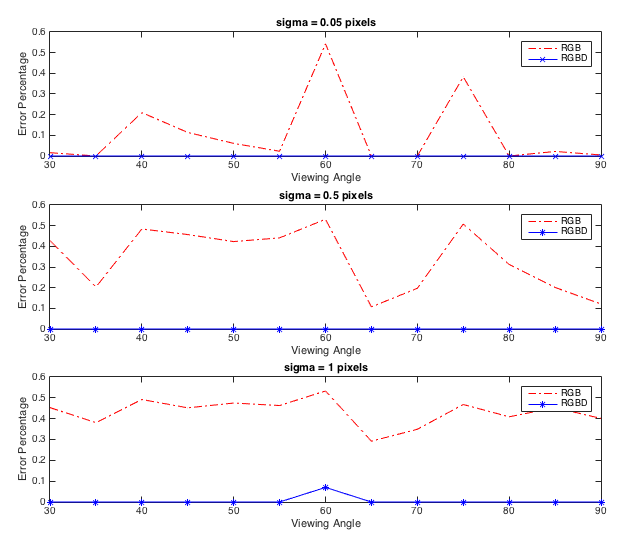
\includegraphics[width=\columnwidth]{figs/viewing_angle_fig1}
\caption{Viewing Angle vs Error Percentage under different simulated noise level. The new RGBD based algorithm can resist noise in the RGB image and it vastly outperforms the original algorithm.}
\label{fig:viewing_result}
\end{figure}

\begin{figure}
\centering
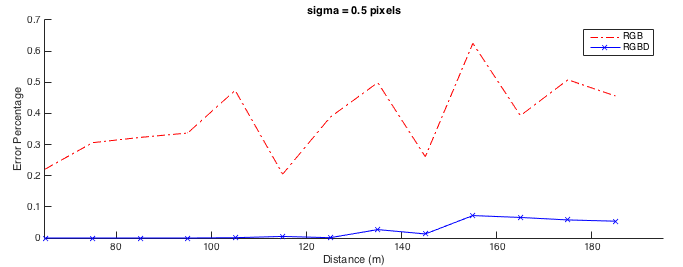
\includegraphics[width=\columnwidth]{figs/distance_fig1}
\caption{Distance vs Error Percentage. Data are captured at a $10$ cm increment from $65$ cm to $185$ cm.}
\label{fig:distance_result}
\end{figure}

\begin{figure}
\centering
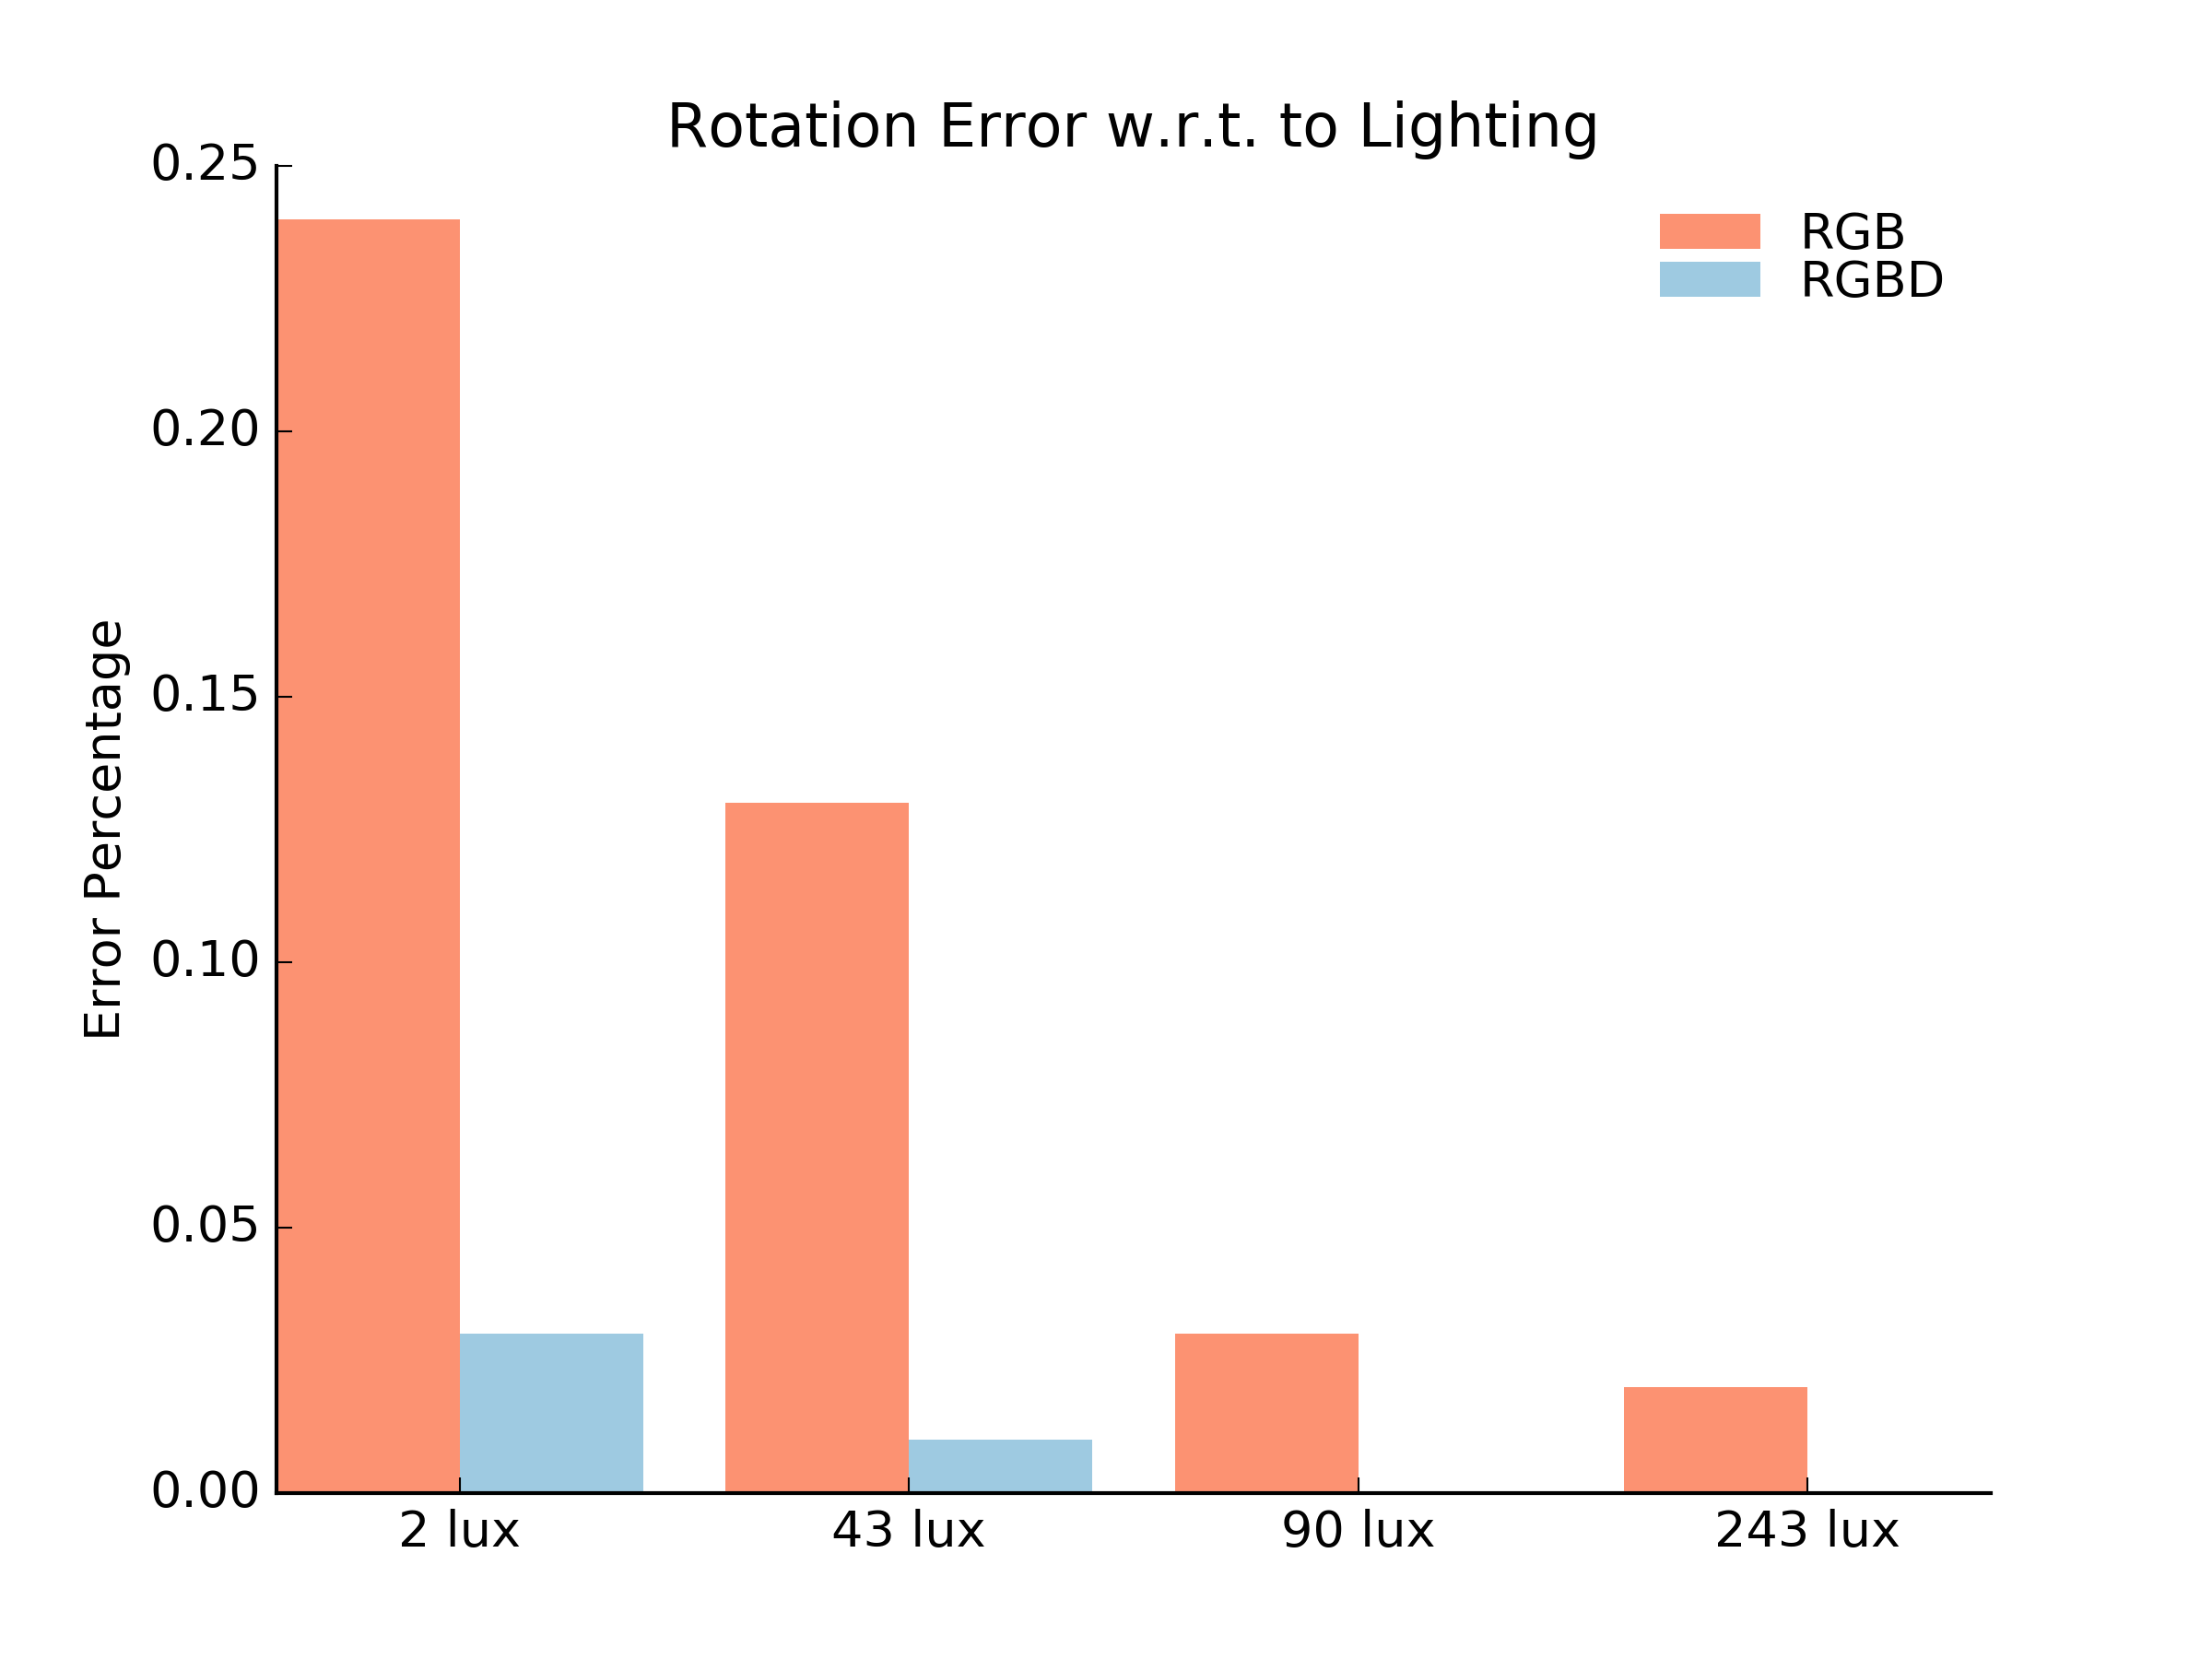
\includegraphics[width=\columnwidth]{figs/lighting_fig1}
\caption{Illumination vs Error Percentage. Data are captured at $65$ cm away from the camera at a $40$ degree angle.}
\label{fig:lighting_result}
\end{figure}
As the result shown in figure 7 indicates, the viewing angle has large effect on the rotation error. As we expected, the empirical results show a very clear bimodal distribution for the Apriltags at different viewing angles. The depth-sensor fused algorithm vastly outperforms the previous algorithm as it is not affected by the perceptual ambiguities. The small amount of the noise introduced to the data only cause a small rotational change around the true pose of the tag. In Figure[8], we threshold all the poses based on their rotational errors and plotted the percentage of unacceptable poses at each viewing point. One interesting observation from the data is that, at most viewing angles, the magnitude of noise above a certain threshold has little effect on the localization accuracy. At most viewing angles, relatively small noises causes a significant accuracy decrease. 

\subsection{Distance}
In additional to the viewing angle, we captured the images at different distances away from the camera at a fixed angle. Figure \ref{fig:distance_result} shows the experiment results.

The relationship between the distance and localization accuracy is much more apparent. As the tag moves further away from the sensor, the number of pixels on the tag decreases. The perspective ambiguity effect becomes more apparent when there is only a small patch of pixels on the tag. However during the experiment, it is difficult to keep the viewing angle precisely consistent at each trail. Therefore, the pose error percentage using RGB is not increasing smoothly in Figure \ref{fig:distance_result}.

We see a clear increase in error percentage in the proposed method when the tag is far away from the camera. This is contributed both by a smaller tag patch size in the depth image and an increasing in noise with the Kinect sensor at a further distance. In these cases, the variance of the depth plane estimation became very wide and the algorithm is unable to converge to the correct pose. The Nevertheless, our method has a significant gain in accuracy at every distance.

\subsection{Lighting}
From our past observations, poor lighting condition is the most significant contributing factor to sensory noise and it results in low localization accuracy. The Kinect V2 sensor used in our experiments dynamically adjust the exposure time under low lighting conditions. The images produced contain very noticeable noise as shown in Figure \ref{}.

Therefore, we also tested the algorithm under harsh lighting conditions in a real world setting. The data were captured under 4 different lighting conditions: 20 lux (dark), 43 (lux) dim, and (90 lux) normal, 243 lux (bright). As results shown in Figure \ref{fig:lighting_result}, the localization accuracy significantly improves with better illumination. 

The Kinect sensor automatically adjusts the exposure settings to compensate for the low lighting. The pictures captured in the dark rooms still appears bright but much more grainy and apparent Gaussian noise in the image. Depth sensor and RGB sensor works optimally under different lighting conditions. In the dark setting, the depth sensor performs well. 


\begin{figure*}
\centering
\subfloat[RGB Image at 75$^{\circ}$]{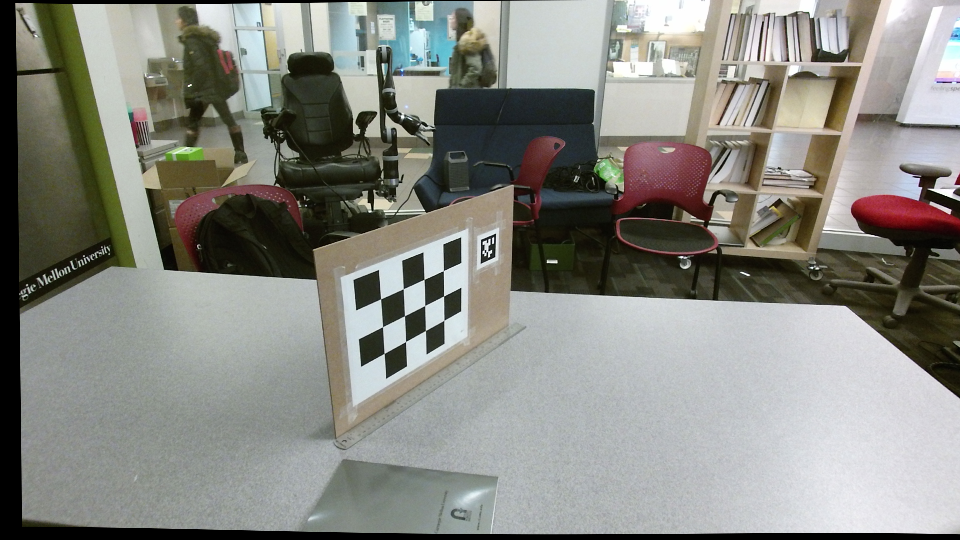
\includegraphics[width=\columnwidth, height=160px]{figs/result_figs/rgb_frame0001} \label{RGB image}}
\subfloat[Distrubtion]{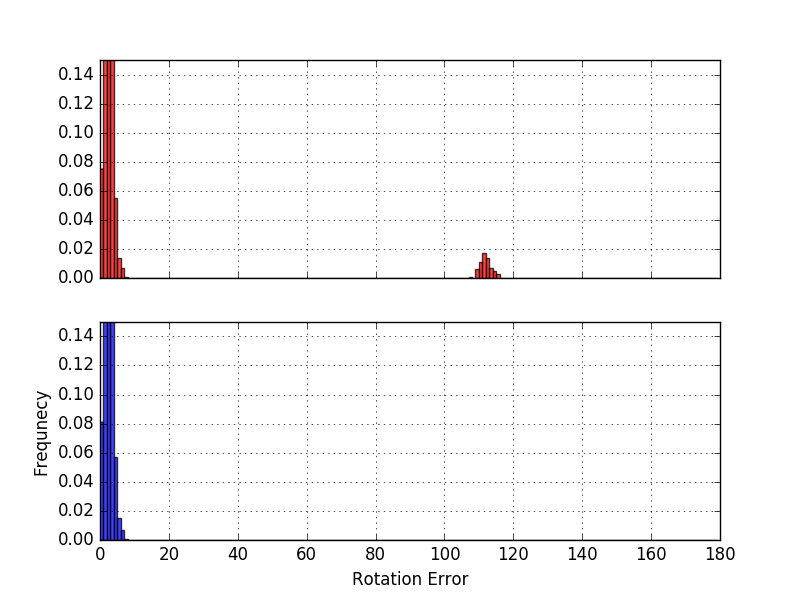
\includegraphics[width=\columnwidth, height=170px]{figs/result_figs/result_0001} \label{RGB image}}
\hfil
\subfloat[RGB Image at 40$^{\circ}$]{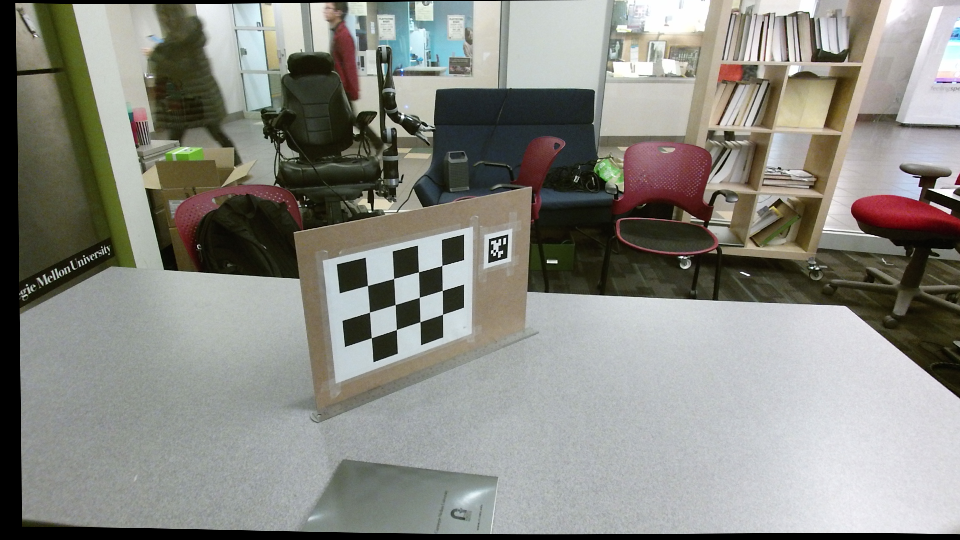
\includegraphics[width=\columnwidth, height=160px]{figs/result_figs/rgb_frame0005} \label{RGB image}}
\subfloat[Close]{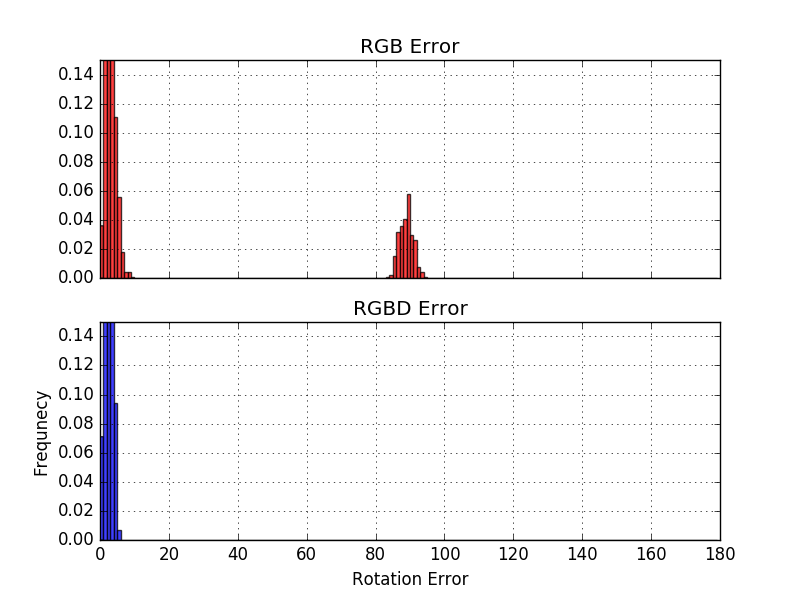
\includegraphics[width=\columnwidth, height=170px]{figs/result_figs/result_0005} \label{RGB image}}
\hfil
\subfloat[RGB Image at 5$^{\circ}$]{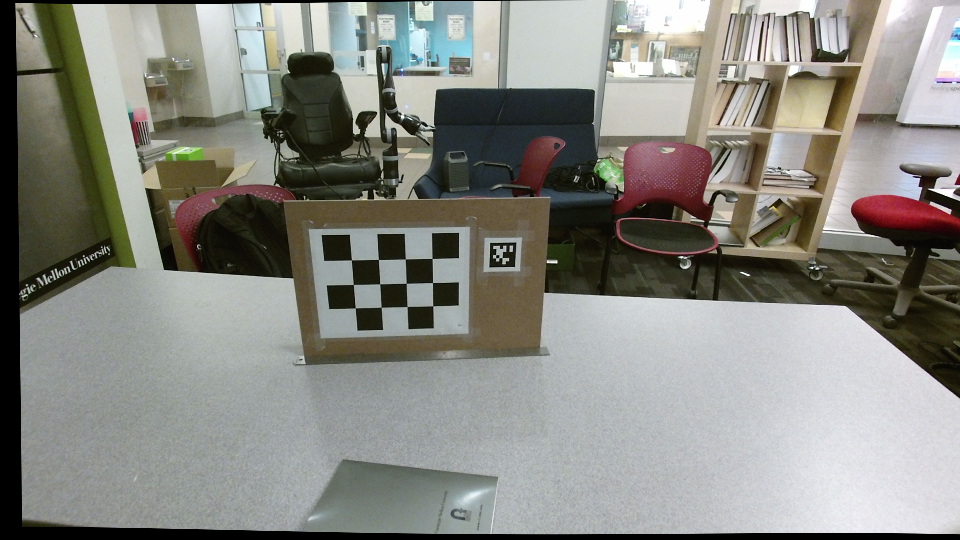
\includegraphics[width=\columnwidth, height=160px]{figs/result_figs/rgb_frame0009} \label{RGB image}}
\subfloat[Close]{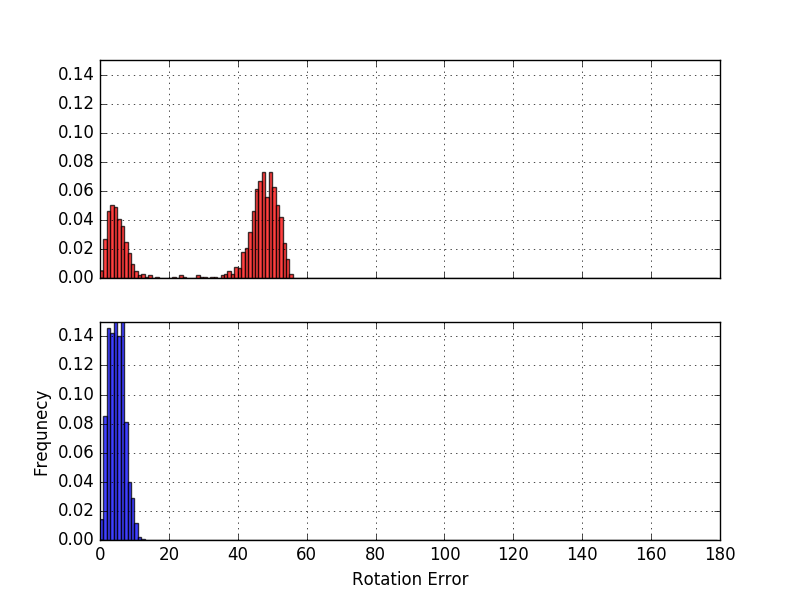
\includegraphics[width=\columnwidth, height=170px]{figs/result_figs/result_0009} \label{RGB image}}
\caption{The fiducial tag plane captured by the depth sensor}
\label{fig:exp_setup}
\end{figure*}
